% Printed 488; principal PDF 495; Google PDF 499.
\par\clearpage
\noindent\makebox[0pt][l]{\fontsize{13}{16}\selectfont 488}\hfill{\small\textbf{NACHLASS.}}\hfill\null\par\medskip
\noindent paar dritten Ranges für die Recognoscirungen gebraucht. Die Messungen mit jenem habe ich alle auf mich allein genommen.

\par\noindent\hspace*{\parindent}Bei dem neuen unmittelbar die Landesgeographie angehenden Geschäft, wobei eine Menge secundärer und tertiärer Messungen gemacht werden müssen, werden daher auch mehrere Theodolithen vom zweiten und dritten Range beständig zu gebrauchen sein. Einen Theodolithen vom zweiten Range (welchen die Sternwarte seit 1813 besitzt) hat der Hr. Hauptmann \textsc{Müller} im vorigen Sommer benutzt, eigentlich damit seine ersten Übungen gemacht. Einen andern (aber nicht ganz befriedigenden) besitzt Hr. Lieutenant \textsc{Hartmann} selbst, der damit im vorigen Jahre seine Messungen gemacht hat. Einen englischen Theodolithen dritten Ranges, auch nicht besonders gut und öftern Derangements unterworfen, benutzte mein Sohn, der sonst, wenn noch einer zweiten Ranges vorhanden gewesen wäre, solchen auch mit Vortheil hätte benutzen können.

\par\noindent\hspace*{\parindent}Ein zweckmässigerer Theodolith dritten Ranges war von mir schon im Frühjahr 1828 in München bestellt; er ist im Herbst angelangt, kostet nur eine sehr geringfügige Summe, und wird doch bei untergeordneten Arbeiten und zum Recognosciren viel brauchbarer sein, als der vorhin erwähnte englische. Einen ähnlichen hat zu gleicher Zeit der Hr. Hauptmann \textsc{Müller} durch meine Vermittelung acquirirt. Für die Recognoscirungsarbeiten ist daher, insofern das Personal nicht vergrössert wird, hinlänglich gesorgt.

\par\noindent\hspace*{\parindent}Für die Messungen des zweiten Ranges sind aber bisher viel zu wenig Hülfsmittel vorhanden. Ich habe daher schon im Herbst noch einen 8-zölligen Theodolithen bestellt, dessen Ablieferung für den April d. J. wenigstens versprochen ist.

\par\noindent\hspace*{\parindent}Was nun aber die Messungen ersten Ranges betrifft, die ich bisher allein auf mich genommen habe, so hoffe ich, dass es späterhin möglich sein wird, auch die andern Officiere nach und nach zu solchen feinern Arbeiten einzuüben, wo dann höchst wünschenswerth und für die Arbeiten förderlich sein wird, wenn wenigstens zwei taugliche Instrumente dazu verwandt werden können. Ich würde daher schon im vorigen Herbst ausser der Bestellung des 8-zölligen Theodolithen zugleich noch auf einen 12-zölligen Bestellung gegeben haben, wenn ich nicht schon damals die Aussicht gehabt hätte, einen solchen 12-zölligen Theodolithen auf andere Weise herbeiziehen zu können,

% Printed 489; principal PDF 496; Google PDF 500.
\par\clearpage
\noindent\null\hfill{\small\textbf{MESSUNGSFEHLER.}}\hfill\makebox[0pt][r]{\fontsize{13}{16}\selectfont 489}\par\medskip
\noindent ohne den Fonds für das Vermessungsgeschäft in Anspruch zu nehmen. Ich wusste nemlich, dass gewünscht werde, für die Generalstabs-Akademie ein solches Instrument anzuschaffen. Nach verschiedenen deshalb mit Hrn. \textsc{Ertel} in München gepflogenen Anfragen habe ich dann auch in der That auf Ersuchen des Hrn. Oberstlieutenant \textsc{Prott} einen solchen 12-zölligen Theodolithen in München bestellt, der hoffentlich im Laufe des Sommers fertig werden wird, und demnächst in den Händen des Hrn. Hauptmann \textsc{Müller}; wenn derselbe die erforderliche Einübung erhalten haben wird, nützliche Dienste leisten wird.

\par\noindent\hspace*{\parindent}Die Münchener Preise für Instrumente dieser Art sind übrigens äusserst mässig. Der 12-zöllige Theodolith, welchen ich seit 1822 zu allen Winkelmessungen bei der Gradmessung gebraucht habe, kostete nur 800 Gulden (leicht Gold); der 8-zöllige oben erwähnte (freilich in den 16 Jahren \textls[120]{etwas} abgenutzte, aber noch immer sehr brauchbare) damals 400 Gulden. Die beiden von ähnlichen Dimensionen, gegenwärtig für die Generalstabs-Akademie und die trigonometrische Vermessung respective bestellten, werden, da ich dabei in mehrern Beziehungen eine einfachere Einrichtung (unbeschadet der \textls[120]{Hauptsache}) angeordnet habe, respective noch bedeutend geringere Preise haben.

\par\noindent\hspace*{\parindent}Bei einer sehr ins Grosse gehenden Unternehmung ist es allerdings zum raschern Fortschreiten, zum angemessenen Ineinandergreifen, und daher selbst in Rücksicht der Gesammtkosten, sehr zweckmässig, eine sehr ansehnliche Zahl von Theodolithen verwenden zu können. Nach einer Privatnachricht werden im nächsten Sommer in Frankreich 160 Theodolithen in Thätigkeit sein. Allein bei unserm kleinen Lande und bei dem beschränkten Personal, welches zu den trigonometrischen Messungen verwandt werden kann und schon einen gewissen Grad von Einübung hat, glaube ich, dass wir wenigstens vorerst mit den vorhandenen und respective in Arbeit befindlichen Instrumenten uns begnügen können. Es kommt dazu, dass man, wie ich die Ehre gehabt habe, Ihnen mündlich zu sagen, auch im Herzogthum Braunschweig eine trigonometrische Messung beabsichtigt, für welche ich auch bereits einen 12-zölligen Theodolithen bestellt habe, und dass es sich wahrscheinlich so wird einrichten lassen, dass diese Messungen zum gegenseitigen Vortheil in einander eingreifend und sich wechselseitig die Hand bietend arrangirt werden können.
\begin{center}\rule{3.5cm}{.4pt}\end{center}
\noindent\makebox[0pt][l]{\small IX.}\makebox[.86\linewidth][r]{62}\par

% Printed 490; principal PDF 497; Google PDF 501.
\par\clearpage
\noindent\makebox[0pt][l]{\fontsize{13}{16}\selectfont 490}\hfill{\small\textbf{BRIEFWECHSEL.}}\hfill\null\par\bigskip
\begin{center}{\large [Über Messungsfehler.]}\par\bigskip
{\large\textsc{Gauss} an \textsc{Olbers}.\quad Gnarrenburg, Julius 1825.}\end{center}
\par\noindent\hspace*{\parindent}.\ .\ .\ .\ .\ .\enspace Ich sehe nicht ohne Missmuth auf meine 5-jährigen Messungen zurück; ich sehe mich, gegen das Ende derselben, ungefähr in einer solchen Lage und in solchen Gefühlen, wie sie wohl viele, vielleicht die meisten Menschen in Beziehung auf das Erdenleben, wenn sie sich dessen Schluss nähern, haben mögen, mit dem Gefühl, dass, wenn mit den eingesammelten und erst spät zur Reife und Klarheit gekommenen Erfahrungen, mit frischer Kraft und mit der erlernten Würdigung so mancher Dinge von vorn her hätte angefangen werden können, viel mehr Zufriedenheit stattgefunden haben könnte. Was die Messungen betrifft, so halte ich mich jetzt überzeugt:

\par\noindent\hspace*{\parindent}1) dass der so wie der meinige gebaute Theodolith alle Winkel zu klein gibt und zwar im Durchschnitt um eine freilich nur sehr kleine, aber bei der sonstigen Trefflichkeit des Instruments, wenn man nur \textls[120]{unter günstigen} Umständen beobachtet, doch sehr scharf anzugebende Grösse --- von der Grösse der Winkel fast unabhängig; es scheint fast, dass das \textls[120]{erste} Drehen sie hauptsächlich hervorbringt, wo der Zapfen doch immer in gewissem Grade gleichsam festgesogen war ---, die freilich mit dem Abnutzen des Instruments grösser werden mag. Meine Jeverschen Messungen, die recht ex professo angelegt waren, diese Grösse mit zu bestimmen, geben sie $0\overset{\prime\prime}{,}4$, und ich glaube nicht, dass sie um $0\overset{\prime\prime}{,}1$ unrichtig ist. Leider bieten meine frühern Messungen keine so nachdrückliche Bestimmungsmittel dar, da ich, obgleich von Anfang an schon das Dasein dieser Fehlerquelle vermuthend, doch glaubte, sie sei zu klein, um nicht als $=0$ betrachtet werden zu müssen. Hätte ich anstatt einer Gradmessung eine Landesvermessung und damit häufiger Gelegenheit zu einem Gyrus horizontis gehabt, so wäre ich ohne Zweifel früher von dieser Ansicht zurück gekommen. Ich werde künftigen Winter die Grösse für jedes Jahr, so gut es angeht, zu bestimmen suchen. Ich halte mich jetzt überzeugt, dass erstens bei steter Berücksichtigung dieser Grösse, zweitens beim Enthalten von allen Messen, wenn die Umstände nicht günstig sind, und drittens bei Beachtung der beiden andern noch zu erwähnenden Umstände, die Messungen auf Heliotroplicht eine fast unglaubliche Feinheit erhalten können, von der ich

% Printed 491; principal PDF 498; Google PDF 502.
\par\clearpage
\noindent\null\hfill{\small\textbf{MESSUNGSFEHLER.}}\hfill\makebox[0pt][r]{\fontsize{13}{16}\selectfont 491}\par\medskip
\noindent nun leider viel mehr entfernt bleibe. Eine Discussion der in Göttingen 1823 gemachten Messungen gibt mir die obige Grösse $=0\overset{\prime\prime}{,}140$, aber nur mit einem Gewicht von 47 Repetitionen, wobei aber doch der wahrscheinliche Fehler nur fast genau $\pm0\overset{\prime\prime}{,}140$ wird, so dass 1 gegen 1 gewettet werden kann, jene Grösse liege nicht ausserhalb der Grenzen $0$ und $+0\overset{\prime\prime}{,}28$. Die Messungen auf dem Timpenberg 1823 gaben die Grösse $+0\overset{\prime\prime}{,}070$ mit dem Gewicht 28. Darf man sie vereinigen, so wäre der Werth für 1823
\[
+0\overset{\prime\prime}{,}114\ \text{mit dem Gewicht }75.
\]
\par\noindent\hspace*{\parindent}Ich werde nach und nach sämmtliche Stationen berechnen, und dann den Einfluss mit in Rechnung bringen.

\par\noindent\hspace*{\parindent}2) Man sollte nie anders als unter günstigen Umständen beobachten, wo die Luft nicht wallt, kein Wind das Instrument erschüttert, die Aufstellung ganz solide ist. Freilich wird man dann oft in mancher Woche gar nicht beobachten und selten an einem Tage mehr als 1--2 Stunden, hohe Bergstationen vielleicht ausgenommen; dafür aber sind 50 solche Messungen mehr werth, als 500 unter ungünstigen Umständen. \textls[120]{Unsere} Instrumente sind eigentlich, falls ihre Trefflichkeit \textls[120]{ganz} benutzt wird, zu gut für den habituellen Zustand der Atmosphäre; die Fehler durch die Wallungen in letzterer sind zehnfach grösser, als die unvermeidlichen vom Instrument herrührenden. Dasselbe gilt wohl auch von den astronomischen Beobachtungen.

\par\noindent\hspace*{\parindent}3) Wenn es irgend möglich ist, sollen die Heliotroplichter ganz frei erscheinen, wo das aber nicht sein kann, soll \textls[120]{nie zwischen den Fäden}, sondern immer auf einem pointirt werden; durch die Befangenheit der Bisection kann sonst ein in constantem Sinne wirkender und vielleicht auf $1\frac12$ bis $2''$ steigender Fehler entstehen. Dass ein solcher Fehler entstehen kann, habe ich zwar immer vermuthet, aber ohne die Erfahrungen in Langwarden hätte ich nie geglaubt, dass er so gross sei. Ich habe früher öfters auf dem Faden pointirt, aber freilich fast nur, wo das Licht frei erschien, und dann nie einen entschiedenen Unterschied gefunden; ich habe diese Beobachtungsart --- wie ich \textls[120]{jetzt} bedaure --- daher fahren lassen, weil sie mir viel beschwerlicher ist, und ich, im \textls[120]{allgemeinen} auch gewiss mit Recht, glaubte, ich könne auf den Fäden nicht so genau pointiren als dazwischen.

\par\noindent\hspace*{\parindent}4) Bei allem dem aber halte ich mich überzeugt, dass Lateralrefractionen
\par\medskip\noindent\makebox[.86\linewidth][r]{62\textsuperscript{*}}\par

% Printed 492; principal PDF 499; Google PDF 503.
\par\clearpage
\noindent\makebox[0pt][l]{\fontsize{13}{16}\selectfont 492}\hfill{\small\textbf{BRIEFWECHSEL.}}\hfill\null\par\medskip
\noindent existiren, in constantem Sinn bei der zum Beobachten tauglichen Tageszeit, wenn das Licht nahe bei Bäumen etc. vorbei streicht. Die oben bei 1) bis 3) angegebenen Umstände wirken doch in mehrern Dreiecken nicht so stark, um die grossen Anomalien der Winkelsumme zu erklären, und sie würden von der Fehlersumme in dem Dreieck, z. B. Garlste-Lehe-Varel, wo sie $4\overset{\prime\prime}{,}9$ beträgt, schwerlich mehr als $1\frac12$ bis $2''$ abdingen können, und das übrige ist dann noch viel zu gross, um auf die unregelmässigen Messungsfehler geschoben werden zu können. Zu meinem grossen Missvergnügen hat auch gewiss auf der Seite Brillit-Lehe eine solche Seitenrefraction statt und zwar in dem Sinn, dass auch hier die Winkel zu klein werden; der sehr kostspielige Durchhau ging anfangs zu weit links, er wurde noch etwas erweitert, dass Lehe hier sichtbar wurde, aber so hart an der rechten Wand, dass gewiss eine Lateralrefraction stattfindet; ich werde versuchen, einige vortretende dicklaubige Zweige auffinden und wegnehmen zu lassen; es ist aber ungewiss, ob sie aufgefunden werden, und selbst dann bleibt es noch sehr knapp an der rechten Wand. Leider ist auf alle Fälle höchst wahrscheinlich der Winkel in Lehe davon schon stark afficirt, und ungern möchte ich noch einmal dahin zurück; es sei dann, dass es möglich wäre, Bremervörde, welches in Lehe sichtbar sein soll, in Brillit und in Zeven sichtbar zu machen; leider scheint aber ausser Obstbäumen auch ein Bauernhaus in der Richtung Brillit-Bremervörde zu stehen, obwohl ich dies noch nicht gewiss weiss, da ich noch keine Mittel habe, das Azimuth mit einiger Sicherheit anzugeben. Sonst bin ich gewiss, dass diese neue Verbindung sehr viel neues Licht verbreiten würde. Der Winkel in Brillit zwischen Zeven und Bremen scheint sich um $2''$ bessern, d. i. vergrössern, zu wollen, wodurch die Fehlersumme von $4\frac12{}''$ auf
\begin{center}
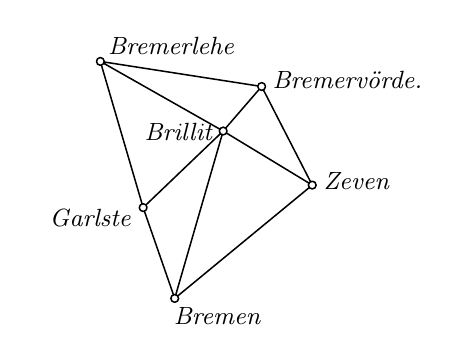
\begin{tikzpicture}[x=.0055cm,y=-.0055cm,line width=.55pt,line cap=round,line join=round,
 every node/.style={font=\small\itshape,inner sep=1pt}]
\path[use as bounding box] (0,0) rectangle (930,700);
\coordinate (Lehe) at (168,78); \coordinate (Voerde) at (541,136);
\coordinate (Brillit) at (452,239); \coordinate (Zeven) at (658,364);
\coordinate (Garlste) at (267,416); \coordinate (Bremen) at (340,626);
\draw (Lehe)--(Voerde)--(Zeven)--(Bremen)--(Garlste)--(Lehe)
 (Lehe)--(Brillit)--(Zeven) (Voerde)--(Brillit)--(Garlste) (Brillit)--(Bremen);
\foreach \v in {Lehe,Voerde,Brillit,Zeven,Garlste,Bremen}
 \draw[fill=white] (\v) circle[radius=1.4pt];
\node[anchor=south west] at (178,70) {Bremerlehe};
\node[anchor=south west] at (558,148) {Bremervörde.};
\node[anchor=east] at (434,240) {Brillit};
\node[anchor=west] at (676,354) {Zeven};
\node[anchor=east] at (246,439) {Garlste};
\node[anchor=north west] at (330,638) {Bremen};
\end{tikzpicture}
\end{center}
\noindent $2\frac12{}''$ kommt; aber ganz kann dieser Überrest gewiss auch nicht auf die Mes-

% Printed 493; principal PDF 500; Google PDF 504.
\par\clearpage
\noindent\null\hfill{\small\textbf{MESSUNGSFEHLER.}}\hfill\makebox[0pt][r]{\fontsize{13}{16}\selectfont 493}\par\medskip
\noindent sungsfehler kommen, namentlich ist in Bremen der obige Fehler 1) durch das Vor- und Rückwärtsmessen fast ganz eliminirt, und die Pointirungsart kann auch wenig Einfluss haben, da bei der bedeutenden Entfernung und der gewöhnlichen Unsichtbarkeit der Thürme die Lichter so gut wie frei erschienen.\par
\noindent .\ .\ .\ .\ .\ .
\begin{center}{\large\textsc{Gauss} an \textsc{Schumacher}.\quad Göttingen, 14. August 1825.}\end{center}
\par\noindent\hspace*{\parindent}.\ .\ .\ .\ .\ .\enspace Bedeutende Anomalien in meinen Messungen haben mich diesen Sommer sehr gequält: ich bin zwar jetzt überzeugt, dass in den flachen Gegenden beim harten Wegstreichen über oder neben Holz starke Lateralrefractionen stattfinden können, die in den zum Messen tauglichen Stunden immer in Einem Sinn wirken; allein eben so gewiss ist’s, dass sie sich mit andern Fehlerquellen gemischt haben, denen ich jetzt ziemlich auf die Spur gekommen bin. Besonders folgenden beiden.\quad 1) Das Pointiren bei Heliotroplicht \textls[120]{zwischen} den Fäden, zumal auf schwaches, taugt nicht, wenn es nicht frei ist, sondern z. B. in der Laterne eines Thurms, die selbst ziemlich gut sichtbar ist, excentrisch sich befindet: es können daher constante Fehler von mehr als $2''$ entstehen; ich habe, seitdem ich mich davon überzeugt habe, in solchen Fällen immer auf einem Faden pointirt, und dadurch zum Theil bedeutende Verminderung der Anomalien erhalten.\quad 2) Der Theodolith, so gebaut wie die unsrigen, gibt entschieden alle Winkel zu klein, und der Durchschnittswerth des Fehlers (der von der Grösse des Winkels wenig abhängig zu sein scheint) lässt sich mit vieler Schärfe bestimmen, mag aber, wie das Instrument sich immer mehr abnutzt, immer zunehmen. In Brillit fand ich $0\overset{\prime\prime}{,}723$, wobei der wahrscheinliche Fehler unter $0\overset{\prime\prime}{,}1$ sein wird. In Jever hatte ich nur etwa $0\overset{\prime\prime}{,}5$. Ich bin noch nicht gewiss, ob die Hauptquelle des Fehlers in der Hemmung des Limbuskreises (besonders der Kugel) oder in der Hülse, die das untere Fernrohr trägt, oder der Schraube, die sie gegen den Fuss des Instruments hält, liegt; letztere ist an meinem Instrument ziemlich ausgenutzt, und ich lasse jetzt, um Versuche zu machen, die Hemmung des Limbuskreises unmittelbar an den Fuss des Instruments anbringen, wobei ich das untere Fernrohr ganz wegnehmen werde; ich halte solches nicht blos für unnütz, wo man eine solide Aufstellung hat, sondern für nachtheilig, insofern seine Hülse, als Zwischeninstanz zur Befestigung des

% Printed 494; principal PDF 501; Google PDF 505.
\par\clearpage
\noindent\makebox[0pt][l]{\fontsize{13}{16}\selectfont 494}\hfill{\small\textbf{BRIEFWECHSEL.}}\hfill\null\par\medskip
\noindent Limbuskreises an den Fuss, die Gefahr von Beweglichkeit des Limbuskreises, während er fest vorausgesetzt wird, vervielfältigt. Ich hätte sehr gewünscht, über diese Gegenstände einmal recht ausführlich mit Ihnen zu sprechen und meine Erfahrungen und Ansichten gegen die Ihrigen auszutauschen.
\par\bigskip
\begin{center}{\large\textsc{Gauss} an \textsc{Bessel}.\quad Göttingen, 29. October 1843.}\end{center}
\par\noindent\hspace*{\parindent}.\ .\ .\ .\ .\ .\enspace Es handelt sich um eine Erfahrung, die mich oft gequält hat, nemlich die, dass die Theodolithen nach \textsc{Reichenbach}s Construction die Tendenz haben, alle Winkel zu klein zu geben. Vielleicht haben Sie ähnliche Erfahrungen gemacht, die ich gern gegen die meinigen austauschen möchte.

\par\noindent\hspace*{\parindent}Bei meinen Winkelmessungen zur Gradmessung 1821 bis 1823 und bei der nachherigen Erweiterung meiner Dreiecke 1824 und 1825 habe ich zwei verschiedene 12-zöllige Theodolithen gebraucht (Verniers $4''$ gebend, Vergrösserung etwa 35-mal), den einen, welchen \textsc{Schumacher} mir borgte, von \textsc{Reichenbach} selbst, bloss im Jahre 1821, den andern von \textsc{Ertel}, welcher jenem ganz gleich und der Eigenthum der Sternwarte ist, 1822 bis 1825. An dem ersten habe ich die Erscheinung gar nicht bemerkt, an dem andern in den ersten drei Jahren und Anfangs 1825 auch nicht; erst in der letzten Hälfte der Messungen bemerkte ich sie, zwar nur in geringer Grösse, aber doch so entschieden, dass nicht daran gezweifelt war. Eine Erklärung, wenigstens der Hauptquelle, liegt nun allerdings nahe genug. Zur Abkürzung nenne ich $A$, $B$ die beiden Objecte und setze voraus, dass $B$ rechts von $A$ liegt, und dass immer die erste Pointirung $A$, die zweite $B$ gilt. Nachdem man abgelesen und auf $A$ eingestellt hat, löst und bewegt man die Alhidade, um $B$ zu erreichen. Allein die Voraussetzung, dass während dieser Bewegung der Kreis selbst \textls[120]{absolut} fest steht, ist allerdings precär; existirt die geringste für sich nicht erkennbare Unfestigkeit, so wird die Drehung der Alhidade den Kreis ein klein wenig in demselben Sinn (von links nach rechts) mitdrehen: der Ablesungsunterschied wird also den Winkel zu klein geben. Bei einer auch noch so grossen Anzahl von Repetitionen wird das Endresultat immer zu klein bleiben.

\par\noindent\hspace*{\parindent}Ich habe, als ich dies erkannt hatte, (in Jever) das Auskunftsmittel ergriffen, zu einer Anzahl von auf gewöhnliche Art gemachten Repetitionen

% Printed 495; principal PDF 502; Google PDF 506.
\par\clearpage
\noindent\null\hfill{\small\textbf{MESSUNGSFEHLER.}}\hfill\makebox[0pt][r]{\fontsize{13}{16}\selectfont 495}\par\medskip
\noindent immer ebenso viele hinzu zu setzen, wo ich\ \raisebox{1.5ex}{\scriptsize.}\ die Alhidade von rechts nach links durch das Supplement zu $360^\circ$ bewegte. Hier wurden nun immer alle Winkel grösser als vorher, und der Unterschied, durchschnittlich gegen 2 Secunden betragend, schien gar nicht oder wenigstens nicht merklich von der Grösse der Winkel abzuhängen. Das Mittel beider Resultate konnte also für den wahren Werth des Winkels gelten, und in der That waren alle auf diese Art, sowohl auf dieser Station wie auf den übrigen, gewonnenen Resultate vollkommen befriedigend. Es schien also, dass dieser Theodolith in seinem damaligen Zustande alle auf gewöhnliche Art gemessenen Winkel gegen eine Secunde zu klein gab.

\par\noindent\hspace*{\parindent}Die Bewegung des ganzen Kreises vom ersten Ablesen bis zum ersten\linebreak
Pointiren, nachher vom \begin{tabular}[c]{@{}c@{}}2.\\4.\\6.\end{tabular}\ etc. zum \begin{tabular}[c]{@{}c@{}}3.\\5.\\7.\end{tabular}\ etc. Pointiren, wurde immer von der\linebreak
rechten nach der linken gemacht (durch den Winkel $<180^\circ$); allerdings ist es wenigstens denkbar, dass auch hier ein Einfluss in constantem Sinn stattfinden kann. Liegt nemlich die Unfestigkeit zum Theil in den Stellschrauben, Muttern, Kugeln, so kann auch, während der ganze Kreis sich dreht, in Folge der Reibung des Alhidadenzapfens auf den ihn unten unterstützenden Federn eine kleine Verstellung der Ablesung stattfinden, welche dann gerade die umgekehrte Wirkung hat, also zur Vergrösserung der Winkel beitragen würde. Ich habe aber vorausgesetzt, dass dieser Einfluss unmerklich sei. Es würde einen sehr grossen Zeitaufwand kosten, a posteriori darüber Aufschluss zu erhalten. Ich brauche nicht zu erinnern, dass ich \textls[120]{stets} dafür gesorgt habe, dass die Stellschrauben nicht zu leicht gingen.

\par\noindent\hspace*{\parindent}An irgend einer Unfestigkeit muss es ohne Zweifel liegen, aber es ist schwer auszumitteln, wo hauptsächlich. Ich habe nachher an diesem Theodolithen eine Abänderung machen lassen, um diejenige Unfestigkeit, die denkbarer Weise bei derjenigen Drehungsbewegung stattfinden könnte, vermittelst welcher man das Versicherungsfernrohr bewegt, weg zu schaffen. Ich habe nemlich das bei fester Aufstellung ganz unnütze Versicherungsfernrohr ganz weggeworfen und den Arm, an welchem die Kreishemmung ist, durch starke Kniestücke unmittelbar mit dem Fuss verbinden lassen. Allein nach dieser Veränderung sind zu wenige Messungen mit diesem Instrument gemacht, um über den Effect sicher urtheilen zu können.

% Printed 496; principal PDF 503; Google PDF 507.
\par\clearpage
\noindent\makebox[0pt][l]{\fontsize{13}{16}\selectfont 496}\hfill{\small\textbf{BRIEFWECHSEL.}}\hfill\null\par\medskip
\par\noindent\hspace*{\parindent}Bei den spätern Messungen von 1828 bis 1843 sind von meinen Officieren drei andere Theodolithen gebraucht.
\par\noindent\hspace*{\parindent}1) von \textsc{Hartmann} ein 8-zölliger \textsc{Reichenbach}scher Theodolith, schon seit 1813 im Besitz der Sternwarte;
\par\noindent\hspace*{\parindent}2) von \textsc{Müller} ein 12-zölliger \textsc{Ertel}scher Theodolith, dem hannoverschen Generalstab gehörend (von mir besorgt), dem obigen ganz ähnlich, aber ohne Höhenkreis und Versicherungsfernrohr;
\par\noindent\hspace*{\parindent}3) von meinem Sohn ein 8-zölliger \textsc{Ertel}scher Theodolith, auch ohne Höhenkreis und Versicherungsfernrohr, aber das Fernrohr ganz von derselben Stärke wie bei Nr. 2. Der Vernier gibt hier $10''$.

\par\noindent\hspace*{\parindent}An Nr. 1 hat sich das Phänomen nicht bemerklich gemacht; das Instrument ist übrigens nur ein paar Jahre gebraucht; die Winkelresultate fielen immer recht sehr gut aus. Das Fernrohr ist von schwächerer optischer Kraft, aber \textsc{Hartmann} hatte immer ein anderes stärkeres Fernrohr eingelegt, welches ihm selbst gehörte. Ich erwähne diesen Umstand bloss, um zu erklären, warum dieser Theodolith nachher nicht mehr gebraucht ist.

\par\noindent\hspace*{\parindent}Über Nr. 2 schreibe ich jetzt bloss aus dem Gedächtniss und kann in diesem Augenblick nicht genau sagen, wann das Phänomen angefangen hat, sich zu zeigen. Irre ich nicht, so ist in den ersten Jahren keine besondere Spur davon erschienen, aber in den spätern war es unverkennbar und wenigstens doppelt so gross, wie an dem von mir gebrauchten Instrument. Jenes ist oft zerlegt, gereinigt, auch, wenn ich mich recht erinnere, mit neuen Stellschrauben von \textsc{Hohnbaum} in Hannover versehen, ohne den Fehler zu heben. Ich habe dem seligen \textsc{Müller} immer das oben erwähnte Mittel dringend empfohlen; ich glaube aber nicht, dass er es immer consequent angewandt hat.

\par\noindent\hspace*{\parindent}Mit Nr. 3 hat mein Sohn in den Jahren 1829, 1830, 1831, 1833 sehr ausgedehnte Messungen ausgeführt; die Winkel (beiläufig gesagt, an jeder Station werden in der Regel \textls[120]{alle} Combinationen zwischen allen Hauptrichtungen gemessen, wie Sie auch aus \textsc{Gerling}s Arbeiten sehen können) stimmten immer zu meiner vollen Zufriedenheit, wenigstens ebenso gut oder fast noch besser, als die \textsc{Müller}schen mit Nr. 2, und der Fehler zeigte sich wenigstens nicht in erheblichem Grade.

\par\noindent\hspace*{\parindent}Von 1834 an ist dieser Theodolith etwa 5 oder 6 Jahr im magnetischen Observatorium, nachher zu Zeiten von \textsc{Goldschmidt} bei Winkelmessungen ge-

% Printed 497; principal PDF 504; Google PDF 508.
\par\clearpage
\noindent\null\hfill{\small\textbf{MESSUNGSFEHLER.}}\hfill\makebox[0pt][r]{\fontsize{13}{16}\selectfont 497}\par\medskip
\noindent braucht, die aber von zu untergeordneter Natur waren, als dass dabei obiger Fehler hätte in Frage kommen können.

\par\noindent\hspace*{\parindent}Diesen selben Theodolithen Nr. 3 hat nun aber mein Sohn im vorigen Sommer wieder bei Hauptwinkeln gebraucht: allerdings waren an den Standpunkten, wo die meisten Winkel gemessen wurden (Thürmen in Hamburg und Stade), die Umstände in vielfacher Beziehung äusserst ungünstig, aber dennoch ging das jetzige Vorhandensein jenes Minusfehlers, und zwar wohl 3 bis $4''$ betragend, auf das entschiedenste hervor. Der Theodolith war vor der Absendung hier gereinigt und nachgesehen, und durchaus keine Unfestigkeit bemerkt. Doch fand mein Sohn das Ende der Stellschraube des Kreises ziemlich ausgeschliffen, und die Beobachtungen der ersten Tage, wo dieser Umstand nicht beachtet war, wurden deshalb verworfen; später wurde der Gebrauch dieses Schraubenstücks sorgfältig vermieden, und es liess sich keine Unfestigkeit daran erkennen. Ich werde den Theodolithen nun wieder hieher kommen lassen und versuchen, ob ich durch Abänderungen dem Fehler oder wenigstens seiner Wirksamkeit nicht abhelfen kann. Ich werde neue Klemmbacken machen lassen; unschlüssig bin ich noch, ob ich ganz neue Schrauben mit Zubehör machen lasse, aus Besorgniss, vom Regen in die Traufe zu kommen. Da Sie selbst einen kleinen Theodolithen von \textsc{Meyerstein} erhalten haben, so bitte ich Sie, gerade \textls[120]{diesen} Theil der Arbeit einer recht sorgfältigen Prüfung zu unterwerfen und mir den Befund vertraulich mitzutheilen. Dann habe ich noch eine Idee zu einem Mittel, welches zwar den Fehler (eine versteckte Unfestigkeit) nicht wegschaffen, aber doch, wie ich hoffe, ihn unschädlich machen kann.

\par\noindent\hspace*{\parindent}Bekanntlich sind Alhidadenzapfen und die Büchse dieses Zapfens, die selbst wieder Limbuskreiszapfen ist, von unten, jedes für sich, auf Federn gestützt. Diese Federn will ich so abändern lassen, dass man mit Leichtigkeit und augenblicklich ihre Spannung nach Gefallen verstärken oder schwächen kann. Mit diesen Spannungsänderungen soll dann während der Messungen immer planmässig abgewechselt werden, so dass, wenn die Alhidade gedreht wird, die Federn, worauf ihr Zapfen sich stützt, stark, die Federn, die die Büchse stützen, fast gar nicht gespannt sind, und umgekehrt, wenn der ganze Kreis gedreht wird. \textsc{Meyerstein} glaubt eine solche Änderung recht zweckmässig einrichten zu können, und ich verspreche mir davon viel Erfolg. Nur schade,
\par\medskip\noindent\makebox[0pt][l]{\small IX.}\makebox[.86\linewidth][r]{63}\par
